
\documentclass[11pt]{article}

\usepackage[a4paper,margin=1in]{geometry}
\usepackage{amsmath,amssymb,amsthm,mathtools}
\usepackage{microtype}
\usepackage{enumitem}
\usepackage{hyperref}
\hypersetup{colorlinks=true,linkcolor=blue,citecolor=blue,urlcolor=blue}
\usepackage{booktabs}
\usepackage{graphicx}
\usepackage{tikz}
\usetikzlibrary{arrows.meta,calc,positioning,shapes.geometric}

\newtheorem{theorem}{Theorem}[section]
\newtheorem{lemma}[theorem]{Lemma}
\newtheorem{proposition}[theorem]{Proposition}
\newtheorem{corollary}[theorem]{Corollary}
\newtheorem{claim}[theorem]{Claim}
\theoremstyle{definition}
\newtheorem{definition}[theorem]{Definition}
\newtheorem{remark}[theorem]{Remark}

\newcommand{\F}{\mathbb F}
\newcommand{\bits}{\{0,1\}}
\newcommand{\RevRes}{\mathrm{RevRes}}
\newcommand{\Fal}{\operatorname{Fal}}
\newcommand{\codim}{\operatorname{codim}}
\newcommand{\supp}{\operatorname{supp}}
\newcommand{\bsupp}{\operatorname{bsupp}}
\newcommand{\Span}{\operatorname{span}}
\newcommand{\rowspan}{\operatorname{rowspan}}
\newcommand{\rank}{\operatorname{rank}}
\newcommand{\E}{\mathbb E}
\newcommand{\Prb}{\mathop{\Pr}}
\newcommand{\poly}{\operatorname{poly}}
\newcommand{\SoPL}{\mathrm{SoPL}}
\newcommand{\SoD}{\mathrm{SoD}}

\title{A Superpolynomial Formula-Size Lower Bound for\\
Reversible Resolution over Parities via a Constant-Size Indexing Lift}
\author{}
\date{}

\begin{document}
\maketitle

\begin{abstract}
We give a formal reduction showing that a short reversible-resolution-over-parities
refutation of a constant-size indexing lift of the Sink-of-DAG contradiction would yield
a low-degree semi-algebraic certificate contradicting the robust approximate
Nullstellensatz lower bound for Sink-of-Potential-Line.
The key new lemma is an exact structural statement about arbitrary affine subspaces
under the $3$-bit indexing gadget: after averaging an affine-subspace indicator over
gadget preimages, one obtains a low-degree conical junta plus a uniformly exponentially
small nonnegative error. Combining this with the pointwise conservation law of
$\RevRes(\oplus)$ gives a lower bound
\[
  \operatorname{Size}_{\RevRes(\oplus)}(\Psi_n)
  \ge 2^{n^{\Omega(1)}}
\]
for a polynomial-size family of CNFs $\Psi_n$. Consequently the lower bound is
$\exp(|\Psi_n|^{\Omega(1)})$, and hence is superpolynomial in the actual encoding size
of the formula.

The only non-elementary imported input is the published
$1/2$-approximate-Nullstellensatz degree lower bound for $\SoPL_n$ and the standard
$\SoPL$-inside-$\SoD$ amplification framework of~\cite{GHJMPRT}.  The affine lifting lemma,
the reversible conservation identity, the robust error-tolerant amplification step,
and the parameter calculation are proved here.
\end{abstract}

\tableofcontents

\section*{Proof overview}
\addcontentsline{toc}{section}{Proof overview}

We begin with a high-level description of the argument and the role of the main
ingredients.  The proof starts from the Sink-of-DAG contradiction $\SoD_{n^2}$,
for which the coefficient-growth argument of~\cite{GHJMPRT} can be driven by the
approximate-Nullstellensatz hardness of $\SoPL_n$.  We then apply a constant-size
indexing gadget to every Boolean variable of $\SoD_{n^2}$ and prove that the resulting
ordinary CNF is hard for $\RevRes(\oplus)$.

The argument has the following conceptual steps.

\paragraph{1. A reversible proof gives an exact pointwise conservation identity.}
Every $\RevRes(\oplus)$ rule preserves, for each Boolean assignment, the number of
falsified clauses on the blackboard.  Consequently, a refutation can be compressed to
an endpoint identity of the form
\[
  \sum_D \alpha_D\,\mathbf 1_{\Fal(D)}
  = q+\sum_j \mathbf 1_{A_j},
\]
where the $D$'s are initial lifted clauses, $q\ge1$ counts final empty clauses, and
each $A_j$ is the affine subspace falsifying a final parity clause.  Thus all of the
intermediate reversible derivation is replaced by one exact identity involving only
initial clauses and affine subspaces.  See Section~\ref{sec:revres}, especially
Proposition~\ref{prop:static}, for the precise conservation argument.

\paragraph{2. Average the identity over preimages of a constant-size indexing gadget.}
For each outer variable $z_i$ we use the three-bit gadget
$z_i=g(s_i,u_i,v_i)$, and for a fixed outer assignment $z$ we sample the internal
assignment $X$ uniformly from the product preimage $g^{-1}(z)$.  The truth-table lift
has a particularly simple behavior under this averaging.  Let $C$ be a base $\SoD$
clause of width $w_C$, let
\[
  a_C(z):=\mathbf 1[C\text{ is falsified by }z],
\]
and let $D_{C,\xi}$ be one of the lifted clauses corresponding to an internal assignment
$\xi$ in the gadget preimage of the unique falsifying assignment of $C$.  Since each
one-bit gadget preimage has exactly four points and the gadget blocks are independent,
\[
  \E_{X\sim\mu_z}\bigl[\mathbf 1_{\Fal(D_{C,\xi})}(X)\bigr]
  =4^{-w_C}a_C(z).
\]
Thus, if $\alpha_{C,\xi}$ is the multiplicity of $D_{C,\xi}$ in the endpoint identity,
all lifted clauses above the same base clause combine into the nonnegative coefficient
\[
  \lambda_C:=4^{-w_C}\sum_\xi\alpha_{C,\xi}\ge0.
\]
On the right-hand side, an affine subspace $A$ contributes exactly the conditional
probability
\[
  h_A(z):=\Pr[X\in A\mid g^N(X)=z].
\]
Therefore averaging the pointwise endpoint identity from Step~1 gives the exact outer
identity
\[
  \sum_C\lambda_C a_C(z)
  =q+\sum_j h_{A_j}(z).
\]
The left-hand side is now a nonnegative linear combination of the original $\SoD$
axiom-falsification polynomials.  Hence the entire lifting problem has been reduced to
understanding the functions $h_A$ arising from affine subspaces on the internal gadget
variables.  See Section~\ref{sec:averaging} for the lifted CNF and the full averaging calculation.

\paragraph{3. Decompose every affine preimage-density into a conical low-degree part
and a tiny positive error.}
Fix a threshold $R$, and write
\[
  r:=\operatorname{codim}(A),
\]
so $r$ is the number of independent affine equations defining the nonempty affine
subspace $A$.  We split into two explicit cases.  By ``large codimension'' we mean
precisely
\[
  r>R/4.
\]
In this case the affine-mass bound for the indexing gadget gives, uniformly for every
outer assignment $z$,
\[
  h_A(z)\le 2^{-\kappa_0 r}
  \le 2^{-\kappa_0R/4}
  =2^{-\Omega(R)}.
\]
Thus we may put the entire function into the error term, taking $J_A=0$ and
$E_A=h_A$.

It remains to consider the complementary low-codimension case $r\le R/4$.  We expose
the selector bits of the gadget.  For all but at most a $2^{-R/4}$ fraction of selector
patterns, the remaining consistency conditions depend on at most $R$ outer coordinates;
for those good selector patterns the conditional density is therefore an exact
nonnegative $R$-junta.  Averaging the good contributions gives $J_A$, while the bad
selector patterns contribute the nonnegative error $E_A$.  This gives the exact
decomposition
\[
  h_A=J_A+E_A,
  \qquad
  \deg J_A\le R,
  \qquad
  J_A\ge0,
  \qquad
  0\le E_A\le 2^{-\Omega(R)},
\]
where $J_A$ is a conical junta.  The nonnegativity of the error is important: the
later amplification argument only needs a uniform upper bound on the error and never
needs to control its degree.  See Section~\ref{sec:indexing-lift}, especially
Lemma~\ref{lem:affine-conical}, for the affine-mass and decomposition arguments.

\paragraph{4. A short $\RevRes(\oplus)$ proof therefore yields a robust
semi-algebraic identity for $\SoD$.}
Recall the endpoint identity from Step~1.  Let $q\ge1$ be the number of empty clauses
on the final blackboard; dividing by $q$ normalizes the constant term to $1$.  After
removing clause occurrences that are simply carried unchanged through the proof, let
$A_1,\ldots,A_T$ be the affine subspaces falsifying the remaining nonempty final
parity clauses.  The number of these clauses satisfies $T=O(S)$, where $S$ is the size
of the original reversible proof.

For each $A_j$, Step~3 gives a decomposition
\[
  h_{A_j}=J_j+E_j,
\]
where $0\le J_j(z)\le1$ and $0\le E_j(z)\le2^{-\Omega(R)}$ for every outer assignment
$z\in\{0,1\}^N$.  After dividing the endpoint identity by $q$, set
\[
  J:=\frac1q\sum_{j=1}^T J_j,
  \qquad
  E:=\frac1q\sum_{j=1}^T E_j.
\]
This gives
\[
  P(z)=1+J(z)+E(z),
\]
where $P$ is a nonnegative combination of the $\SoD$ clause-falsification polynomials
and $J$ is a degree-$R$ conical junta.  Since $q\ge1$ and $T=O(S)$, for every
$z\in\{0,1\}^N$ we have
\[
  0\le E(z)\le O(S)\,2^{-\Omega(R)}
  \qquad\text{and}\qquad
  0\le J(z)\le O(S).
\]
In particular,
\[
  \max_{z\in\{0,1\}^N}J(z)\le O(S).
\]
Thus any later argument forcing $J$ to take an exponentially large value immediately
forces the original reversible proof to be large.  See
Section~\ref{sec:short-to-robust} for the full construction and normalization.

\paragraph{5. Apply the robust $\SoD$ coefficient-growth amplification.}
The main amplification step follows the same overall argument as
\cite[Section~5.1]{GHJMPRT}.  At each stage we embed an $\SoPL_n$ instance into one
subgrid of $\SoD$, use the approximate-Nullstellensatz lower bound to make $1+J$
grow by a constant factor, and then redirect the current sinks into a fresh subgrid.
The cleanup removes only a small part of the conical junta, so this growth can be
repeated for many stages.  We need four changes to make that argument work in the
present setting:
\begin{itemize}[leftmargin=2em,itemsep=3pt,topsep=3pt]
\item \emph{We allow a small error term.}
In~\cite{GHJMPRT} the starting identity is exact: $P=1+J$.  Here we have
$P=1+J+E$, where $0\le E\le\eta$.  Thus the lower-bound argument gives a growth
factor $3/2-\eta$ before cleanup instead of $3/2$.  For sufficiently small $\eta$,
the loss in the cleanup is still small enough to leave a fixed factor larger than
$1$; we package the argument as a one-step lemma that keeps a factor $4/3$ from one
stage to the next.

\item \emph{We make the reduction to $\SoPL$ explicit.}
After fixing everything outside the current subgrid, we must apply the
approximate-Nullstellensatz lower bound for $\SoPL$ to the restricted polynomial.
Since our polynomial comes from the lifted $\RevRes(\oplus)$ proof, this does not
follow automatically.  We therefore give an explicit local decision-tree transfer
showing that the restricted polynomial can be written using the canonical $\SoPL$
axioms, with only a small increase in degree.

\item \emph{We use the structured hard family $\mathcal H_n$.}
The cleanup step is simplest on $\SoPL$ instances that are disjoint directed paths
ending in the last row.  We therefore isolate this family as $\mathcal H_n$ and use
the fact that the approximate-Nullstellensatz lower bound is still valid when the
approximation is required only on these inputs.  On such inputs the current solutions
are exactly the last-row sinks that have to be redirected to the next subgrid.

\item \emph{We use the final growth in a different way.}
In~\cite{GHJMPRT}, exponential growth of $J$ is converted into a lower bound on a
Sherali--Adams coefficient.  Here we already know from the reversible endpoint
identity that $\max J\le O(S)$, where $S$ is the size of the original
$\RevRes(\oplus)$ proof.  Therefore exponential growth of $\max J$ directly forces
$S$ to be large.
\end{itemize}
With these changes, the same stage-by-stage iteration gives
\[
  \max_z J(z)\ge 2^{\Omega(n)}.
\]
See Section~\ref{sec:base-lb}, especially Lemma~\ref{lem:robust-sod}, for the full
error-robust amplification argument and its relation to~\cite[Section~5.1]{GHJMPRT}.

\paragraph{6. Finish by a dichotomy on the accumulated error.}
Take $R=n^\beta$ for a sufficiently small constant $\beta>0$.  If
\[
  S\,2^{-\Omega(R)}
\]
is not small, then already $S\ge2^{\Omega(R)}$.  Otherwise the error in the robust
identity is small enough for the amplification theorem, which gives
$\max J\ge2^{\Omega(n)}$; since $\max J\le O(S)$, this again yields
$S\ge2^{\Omega(R)}$.  Thus in all cases
\[
  \operatorname{Size}_{\RevRes(\oplus)}(\Psi_n)
  \ge 2^{n^{\Omega(1)}}.
\]
See Section~\ref{sec:main-proof} for the parameter choice and the final conversion to
formula size.  Finally, the gadget has constant size and the base $\SoD$ clauses have width
$O(\log n)$, so the truth-table lift $\Psi_n$ still has polynomial encoding size.
The lower bound is therefore superpolynomial---indeed stretched exponential---in the
actual size of the CNF.

In summary, the proof may be viewed as the composition
\[
\begin{array}{c}
  \text{short }\RevRes(\oplus)\text{ proof}
  \ \Longrightarrow\ 
  \text{affine endpoint identity}\\[2pt]
  \Longrightarrow\ 
  \text{low-degree conical identity }P=1+J+E\\[2pt]
  \Longrightarrow\ 
  \text{contradiction with robust }\SoD\text{ amplification}.
\end{array}
\]
The only imported lower-bound input is the approximate-Nullstellensatz hardness of
$\SoPL$; the constant-size lifting analysis and the conversion from reversible parity
proofs to the robust conical identity are proved in this paper.


\section{The search principles $\SoD$ and $\SoPL$}\label{sec:search-principles}

We record the two grid search principles used throughout the proof.  This also fixes
our terminology for \emph{active nodes}, \emph{sinks}, and the distinguished source.
The formulations below are the standard ones from~\cite{GHJMPRT}, expressed in the
notation used in this paper.

\subsection{Sink-of-DAG $\SoD_m$}\label{subsec:sod-definition}
The vertices are the $m^2$ grid points
\[
  V=[m]\times[m],
\]
with rows numbered from top to bottom.  The distinguished node is
$d=(1,1)$.  Every node $u=(i,j)$ has a successor datum
$s_u\in[m]\cup\{\mathsf{null}\}$.  For $i<m$, a nonnull value $s_u=k$
means that $u$ points to the node $(i+1,k)$ on the next row; if
$s_u=\mathsf{null}$, then $u$ is \emph{inactive}.  A last-row node is called active
when its successor datum is nonnull; geometrically this is an ``edge leaving the
grid.''  Thus the internal successor pointers form a layered directed acyclic graph
of fan-out at most one, while several nodes are allowed to point to the same node.

A valid $\SoD_m$ output is any one of the following local defects:
\begin{enumerate}[label=(\roman*),leftmargin=2.3em]
\item the distinguished node $(1,1)$ is inactive;
\item some node on the last row is active;
\item an active internal node $u$ points to an inactive node $v$ on the next row.
\end{enumerate}
In case~(iii), the inactive target $v$ is the geometric \emph{proper sink}; in the
canonical search-CNF one may equivalently label the witness by its active predecessor
$u$.  Totality is immediate: if the distinguished node is active, follow successors
row by row.  Either an active node points to an inactive node, or the walk reaches an
active node on the last row.

\begin{figure}[htbp]
\centering
\resizebox{0.92\textwidth}{!}{%
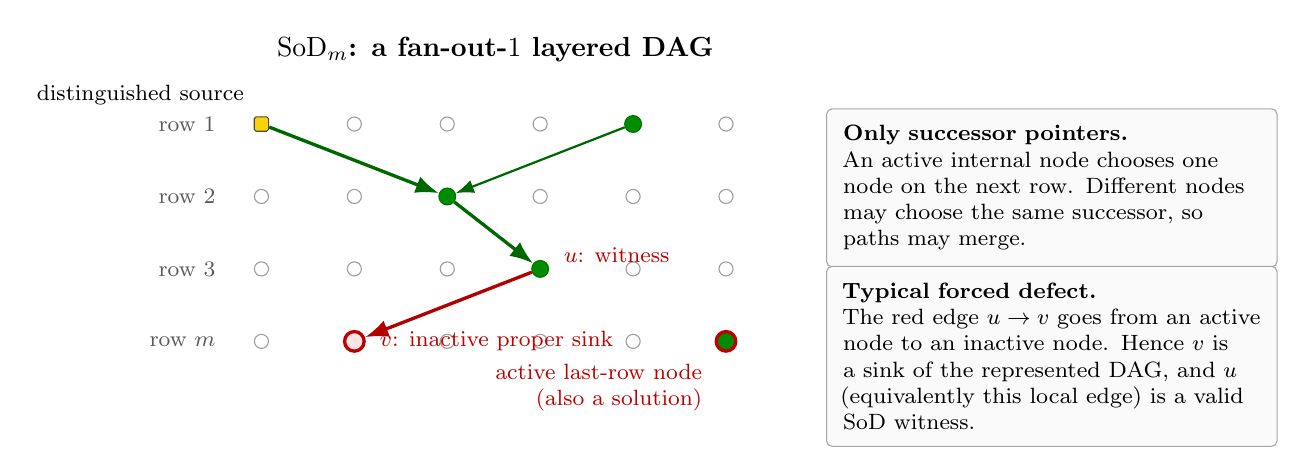
\begin{tikzpicture}[
  >=Latex,
  font=\small,
  gnode/.style={circle,draw=black!38,fill=white,inner sep=1.8pt},
  active/.style={circle,draw=green!45!black,fill=green!55!black,inner sep=2.15pt},
  source/.style={rectangle,rounded corners=0.7pt,draw=black!70,fill=yellow!70!orange,
    minimum width=5.2pt,minimum height=5.2pt,inner sep=1.3pt},
  sinknode/.style={circle,draw=red!75!black,very thick,fill=red!10,inner sep=2.5pt},
  badbottom/.style={circle,draw=red!75!black,very thick,fill=green!55!black,inner sep=2.5pt},
  edge/.style={->,very thick,draw=green!40!black},
  merge/.style={->,thick,draw=green!40!black},
  callout/.style={draw=black!35,rounded corners=2pt,fill=black!2,align=left,inner sep=6pt}
]
% Grid coordinates
\foreach \r in {1,...,4}{
  \foreach \c in {1,...,6}{
    \node[gnode] (S\r-\c) at (1.18*\c,-0.92*\r) {};
  }
}
% row labels
\foreach \r/\lab in {1/{row $1$},2/{row $2$},3/{row $3$},4/{row $m$}}{
  \node[anchor=east,font=\footnotesize,text=black!65] at (0.72,-0.92*\r) {\lab};
}
% active/source overlays
\node[source] (Sd) at (S1-1) {};
\node[active] (Sa) at (S2-3) {};
\node[active] (Sw) at (S1-5) {};
\node[active] (Su) at (S3-4) {};
\node[sinknode] (Sv) at (S4-2) {};
\node[badbottom] (Sb) at (S4-6) {};
% edges, including a merge
\draw[edge] (Sd) -- (Sa);
\draw[merge] (Sw) -- (Sa);
\draw[edge] (Sa) -- (Su);
\draw[edge,draw=red!70!black] (Su) -- (Sv);
% labels
\node[font=\footnotesize,anchor=south east] at ($(Sd)+(-0.10,0.12)$) {distinguished source};
\node[font=\footnotesize,anchor=west,text=red!75!black] at ($(Sv)+(0.20,0)$)
  {$v$: inactive proper sink};
\node[font=\footnotesize,anchor=west,text=red!75!black] at ($(Su)+(0.18,0.18)$)
  {$u$: witness};
\node[font=\footnotesize,anchor=north east,text=red!75!black,align=right]
  at ($(Sb)+(-0.18,-0.16)$) {active last-row node\\(also a solution)};
% fan-in callout
\node[callout,anchor=north west,text width=5.3cm,font=\footnotesize] at (8.35,-0.72)
  {\textbf{Only successor pointers.}\\
   An active internal node chooses one node on the next row.  Different nodes may
   choose the same successor, so paths may merge.};
\node[callout,anchor=north west,text width=5.3cm,font=\footnotesize] at (8.35,-2.72)
  {\textbf{Typical forced defect.}\\
   The red edge $u\to v$ goes from an active node to an inactive node.  Hence $v$ is
   a sink of the represented DAG, and $u$ (equivalently this local edge) is a valid
   $\SoD$ witness.};
% title over grid
\node[font=\bfseries,anchor=south] at (4.15,-0.25) {$\SoD_m$: a fan-out-$1$ layered DAG};
\end{tikzpicture}%
}
\caption{\textbf{The search problem $\SoD_m$.}
Only successor data are present.  Consequently the represented graph can have large
fan-in (the two upper arrows merge), but every active internal node has at most one
outgoing edge.  The distinguished source is shown as a yellow square.  The red local
configuration illustrates the main solution type: an active node points to an
inactive successor.  An inactive distinguished source or an active last-row node is
also a solution.  The drawing is schematic.}
\label{fig:sod-definition}
\end{figure}

The standard binary CNF also denoted $\SoD_m$ is the contradiction asserting that
none of the three solution types above occurs: the distinguished source is active,
every last-row node is inactive, and every successor of an active internal node is
active.  Successor names are encoded in binary, with one code reserved for
$\mathsf{null}$.  Hence the local clauses have width $O(\log m)$.

\subsection{Sink-of-Potential-Line $\SoPL_m$}\label{subsec:sopl-definition}
The vertices are again $[m]\times[m]$ with distinguished node $(1,1)$.  In addition
to successor data $s_{i,j}\in[m]\cup\{\mathsf{null}\}$, every node below the first
row has predecessor data
\[
  p_{i,j}\in[m]\cup\{\mathsf{null}\}.
\]
For $i<m$, we place an \emph{active edge}
\[
  (i,j)\longrightarrow(i+1,k)
  \quad\Longleftrightarrow\quad
  s_{i,j}=k\ne\mathsf{null}
  \ \text{and}\ 
  p_{i+1,k}=j.
  \tag{SP}\label{eq:sopl-active-edge}
\]
An internal node is active exactly when it has such an outgoing active edge.  A
last-row node $(m,j)$ is active when $s_{m,j}\ne\mathsf{null}$.  Because an active
edge requires agreement of the successor and predecessor pointers, every node has
active in-degree and out-degree at most one.  Thus the active graph is a collection
of vertex-disjoint directed paths running downward through the rows.

A valid $\SoPL_m$ output is one of:
\begin{enumerate}[label=(\roman*),leftmargin=2.3em]
\item the distinguished node $(1,1)$ is inactive;
\item some last-row node is active;
\item an inactive node $v$ has an incoming active edge; equivalently, $v$ is a
\emph{proper sink} of one of the active paths.
\end{enumerate}
Starting at an active distinguished source and following the unique active edge, one
must either encounter a proper sink before the last row or arrive at an active
last-row node.  This is the totality principle encoded by $\SoPL_m$.

\begin{figure}[htbp]
\centering
\resizebox{0.92\textwidth}{!}{%
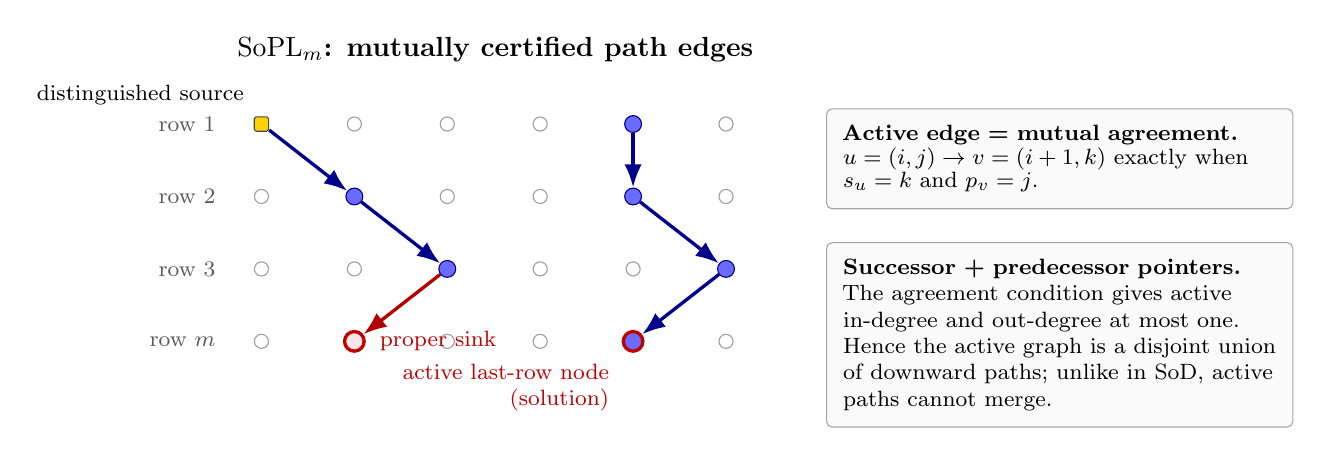
\begin{tikzpicture}[
  >=Latex,
  font=\small,
  gnode/.style={circle,draw=black!38,fill=white,inner sep=1.8pt},
  active/.style={circle,draw=blue!55!black,fill=blue!58,inner sep=2.15pt},
  source/.style={rectangle,rounded corners=0.7pt,draw=black!70,fill=yellow!70!orange,
    minimum width=5.2pt,minimum height=5.2pt,inner sep=1.3pt},
  sinknode/.style={circle,draw=red!75!black,very thick,fill=red!10,inner sep=2.5pt},
  badbottom/.style={circle,draw=red!75!black,very thick,fill=blue!58,inner sep=2.5pt},
  edge/.style={->,very thick,draw=blue!55!black},
  callout/.style={draw=black!35,rounded corners=2pt,fill=black!2,align=left,inner sep=6pt}
]
% Grid
\foreach \r in {1,...,4}{
  \foreach \c in {1,...,6}{
    \node[gnode] (P\r-\c) at (1.18*\c,-0.92*\r) {};
  }
}
\foreach \r/\lab in {1/{row $1$},2/{row $2$},3/{row $3$},4/{row $m$}}{
  \node[anchor=east,font=\footnotesize,text=black!65] at (0.72,-0.92*\r) {\lab};
}
% First path terminating at a proper sink
\node[source] (Pd) at (P1-1) {};
\node[active] (Pa) at (P2-2) {};
\node[active] (Pb) at (P3-3) {};
\node[sinknode] (Pv) at (P4-2) {};
\draw[edge] (Pd) -- (Pa);
\draw[edge] (Pa) -- (Pb);
\draw[edge,draw=red!70!black] (Pb) -- (Pv);
% Second disjoint path ending active on last row
\node[active] (Px1) at (P1-5) {};
\node[active] (Px2) at (P2-5) {};
\node[active] (Px3) at (P3-6) {};
\node[badbottom] (Px4) at (P4-5) {};
\draw[edge] (Px1) -- (Px2);
\draw[edge] (Px2) -- (Px3);
\draw[edge] (Px3) -- (Px4);
% labels
\node[font=\footnotesize,anchor=south east] at ($(Pd)+(-0.10,0.12)$) {distinguished source};
\node[font=\footnotesize,anchor=west,text=red!75!black] at ($(Pv)+(0.20,0)$)
  {proper sink};
\node[font=\footnotesize,anchor=north east,text=red!75!black,align=right]
  at ($(Px4)+(-0.18,-0.16)$) {active last-row node\\(solution)};
% rule callouts
\node[callout,anchor=north west,text width=5.5cm,font=\footnotesize] at (8.35,-0.72)
  {\textbf{Active edge = mutual agreement.}\\[-1pt]
   $u=(i,j)\to v=(i+1,k)$ exactly when\\[-1pt]
   $s_u=k$ and $p_v=j$.};
\node[callout,anchor=north west,text width=5.5cm,font=\footnotesize] at (8.35,-2.42)
  {\textbf{Successor + predecessor pointers.}\\
   The agreement condition gives active in-degree and out-degree at most one.  Hence
   the active graph is a disjoint union of downward paths; unlike in $\SoD$, active
   paths cannot merge.};
\node[font=\bfseries,anchor=south] at (4.15,-0.25) {$\SoPL_m$: mutually certified path edges};
\end{tikzpicture}%
}
\caption{\textbf{The search problem $\SoPL_m$.}
A directed edge is active only when the successor pointer of its tail and the
predecessor pointer of its head agree, as in~\eqref{eq:sopl-active-edge}.  Therefore
the active graph consists of vertex-disjoint downward paths.  The left path terminates
at a proper sink (red); the right path reaches an active last-row node, which is also
a solution.  The distinguished source is the yellow square.  The drawing is
schematic.}
\label{fig:sopl-definition}
\end{figure}

The standard binary CNF $\SoPL_m$ forbids these three outputs: it requires the
distinguished node to be active, all last-row nodes to be inactive, and every node
reached by an active edge to continue with an active outgoing edge.  Both successor
and predecessor names are encoded in $O(\log m)$ bits.  Figure~\ref{fig:sod-definition}
and Figure~\ref{fig:sopl-definition} emphasize the distinction used later in
Section~\ref{sec:base-lb}: $\SoD$ supplies the large ambient layered DAG, whereas an
$\SoPL$ instance can be embedded inside one box as a collection of disjoint paths.

\clearpage

\section{Statement of the result}

We work over $\F_2$ whenever we discuss affine equations.

\begin{theorem}[Main theorem]\label{thm:main}
There exist constants $\varepsilon,c>0$ and an infinite family of unsatisfiable CNF
formulas $\{\Psi_n\}_{n\ge 1}$ such that
\[
  |\Psi_n| \le n^{O(1)}
\]
and every $\RevRes(\oplus)$ refutation of $\Psi_n$ has size at least
\[
  \exp(c n^\varepsilon).
\]
In particular, if $L_n:=|\Psi_n|$ denotes the ordinary bit-size of the CNF encoding,
then for some $\varepsilon'>0$,
\[
  \operatorname{Size}_{\RevRes(\oplus)}(\Psi_n)
  \ge \exp(\Omega(L_n^{\varepsilon'}))
  = L_n^{\omega(1)}.
\]
\end{theorem}

The proof has three ingredients.

\begin{enumerate}[label=(\roman*)]
\item Every $\RevRes(\oplus)$ refutation gives a pointwise identity equating the
weighted number of falsified initial clauses to a positive constant plus indicators
of affine subspaces.
\item For the $3$-bit indexing gadget, the preimage-density function of \emph{every}
affine subspace is a low-degree conical junta plus a uniformly exponentially small
nonnegative error.
\item The coefficient-growth proof for $\SoD$ is robust under such a uniformly small
nonnegative error.
\end{enumerate}

The crucial point for formula size is that the gadget has constant size.  Since the
base $\SoD$ CNF has width $O(\log n)$, its truth-table lift still has polynomial size.

\section{Reversible resolution over parities}\label{sec:revres}

\subsection{Parity clauses and falsifying affine spaces}

A \emph{linear form} is a map
\[
  \ell(x)=a_1x_1\oplus\cdots\oplus a_Nx_N,
  \qquad a_i\in\F_2.
\]
A parity equation is $(\ell=b)$, $b\in\F_2$.
A parity clause is a disjunction
\[
  C=(\ell_1=b_1)\vee\cdots\vee(\ell_t=b_t).
\]
Its falsifying set is
\[
  \Fal(C)
  :=
  \{x\in\bits^N:\ell_j(x)=1-b_j \text{ for all }j\in[t]\}.
\]
Thus $\Fal(C)$ is either empty or an affine subspace of $\F_2^N$.

The empty clause $\bot$ is falsified by every assignment, so
\[
  \mathbf 1_{\Fal(\bot)}\equiv 1.
\]

\subsection{The blackboard system}

We use the reversible blackboard formulation.  The rules are the following, together
with their reverse directions.

\paragraph{Excluded middle.}
\[
  \varnothing
  \longleftrightarrow
  \{(\ell=0)\vee(\ell=1)\}.
\]

\paragraph{Reversible cut.}
\[
 \{A\vee(\ell=0),\,A\vee(\ell=1)\}
 \longleftrightarrow
 \{A\}.
\]

\paragraph{Reversible equivalence.}
One may replace a parity clause $A$ by $B$ whenever
\[
  \Fal(A)=\Fal(B).
\]

A blackboard state is a multiset of parity clauses.  Applying a rule removes one copy
of each premise and inserts one copy of each conclusion.

The only property of the rules needed below is strong soundness.

\begin{lemma}[Pointwise conservation]\label{lem:strong-soundness}
For every application of a $\RevRes(\oplus)$ rule and every Boolean assignment $x$,
the number of falsified clauses in the premise multiset equals the number of falsified
clauses in the conclusion multiset.
\end{lemma}

\begin{proof}
For excluded middle, the introduced clause is a tautology and is never falsified.

For reversible equivalence the two falsifying sets are equal.

For reversible cut, fix $x$.  If $A(x)=1$, none of the three clauses involved is
falsified.  If $A(x)=0$, exactly one of $(\ell=0)$ and $(\ell=1)$ is false, hence
exactly one of
\[
  A\vee(\ell=0),\qquad A\vee(\ell=1)
\]
is falsified.  The clause $A$ is also falsified exactly once.  Thus the falsified
multiplicity is preserved.  The reverse directions preserve the same equality.
\end{proof}

\begin{proposition}[Static endpoint identity]\label{prop:static}
Let $F=\{D_1,\dots,D_M\}$ be a CNF, viewed as parity clauses of rank one.
Suppose a $\RevRes(\oplus)$ refutation starts with
\[
  \mathcal L_0=\biguplus_{i=1}^M \alpha_i\{D_i\}
\]
and ends with a multiset containing $q\ge 1$ copies of $\bot$ and further parity
clauses $B_1,\dots,B_T$.  Then, pointwise on $\bits^N$,
\[
  \sum_{i=1}^M \alpha_i\,\mathbf 1_{\Fal(D_i)}
  =
  q+\sum_{j=1}^T\mathbf 1_{\Fal(B_j)}.
  \tag{2.1}\label{eq:static}
\]
\end{proposition}

\begin{proof}
Apply Lemma~\ref{lem:strong-soundness} successively to every inference step.
The number of falsified clauses is invariant from the initial state to the final
state.  Every copy of $\bot$ contributes one for every assignment.
\end{proof}

\begin{remark}[Removing inert occurrences]\label{rem:inert}
We may assume that every initial clause occurrence participates in some inference and
that every final clause occurrence is either $\bot$ or descends from an inference.
Indeed, an occurrence that is carried unchanged from the initial state to the final
state can be deleted from every blackboard state.

Under any standard Cook--Reckhow encoding, after this reduction the number $T$ of
nonempty final clause occurrences is $O(S)$, where $S$ is the proof size: each such
occurrence must either be created by an inference or be an initial occurrence that
appears as a premise somewhere, and each such event contributes at least a constant
amount to the proof encoding.
\end{remark}

\section{Averaging the endpoint identity over gadget preimages}\label{sec:averaging}

Define the $3$-bit indexing gadget
\[
  g:\bits^3\to\bits,
  \qquad
  g(s,u,v)=
  \begin{cases}
  u,&s=0,\\
  v,&s=1.
  \end{cases}
  \tag{3.1}\label{eq:index}
\]

For each $b\in\bits$,
\[
  |g^{-1}(b)|=4.
\]

For $z=(z_1,\dots,z_N)\in\bits^N$, let $\mu_z$ be the uniform distribution on
\[
  g^{-1}(z)
  :=
  \{X=(X_1,\dots,X_N):g(X_i)=z_i\text{ for all }i\}.
\]
The blocks are independent under $\mu_z$.

A convenient sampling description is:
for each block independently, choose $s_i$ uniformly;
set the selected data bit $y_{i,s_i}=z_i$;
choose the unselected data bit $y_{i,1-s_i}$ uniformly.
Here $y_{i,0}=u_i$ and $y_{i,1}=v_i$.

\subsection{The lifted CNF}

Let
\[
  F_n=\SoD_{n^2}
\]
be the base CNF on outer variables $z_1,\dots,z_N$, where
\[
  N=O(n^4\log n).
\]

For each outer variable $z_i$, introduce a gadget block
\[
  X_i=(s_i,u_i,v_i)
\]
and interpret
\[
  z_i=g(X_i).
\]

Let
\[
  C=\ell_1\vee\cdots\vee\ell_w
\]
be a base clause, and let
\[
  \zeta_C\in\bits^{\operatorname{vars}(C)}
\]
be its unique falsifying assignment on its outer variables.
For every internal assignment
\[
  \xi\in
  \prod_{i\in\operatorname{vars}(C)}g^{-1}(\zeta_C(i)),
\]
introduce the ordinary clause $D_{C,\xi}$ on the $3w$ internal variables which is
falsified exactly by the assignment $\xi$.

Define
\[
  \Psi_n:=F_n\circ g
\]
to be the conjunction of all clauses $D_{C,\xi}$.

\begin{lemma}[Unsatisfiability and size]\label{lem:lift-size}
The CNF $\Psi_n$ is unsatisfiable and has polynomial encoding size:
there is a constant $K$ such that
\[
  |\Psi_n|\le n^K.
  \tag{3.2}\label{eq:polysize}
\]
\end{lemma}

\begin{proof}
Any assignment $X$ to the internal variables induces an outer assignment
\[
  z_i=g(X_i).
\]
Since $F_n$ is unsatisfiable, some base clause $C$ is falsified by $z$.
The restriction of $X$ to the blocks of $C$ is then one particular
\[
  \xi\in\prod_{i\in\operatorname{vars}(C)}g^{-1}(\zeta_C(i)),
\]
and the corresponding lifted clause $D_{C,\xi}$ is falsified.
Thus $\Psi_n$ is unsatisfiable.

If $C$ has width $w$, then it yields exactly $4^w$ lifted clauses, each of width $3w$.
The base formula has polynomially many clauses and width $w=O(\log n)$.
Therefore
\[
  4^w=n^{O(1)},
\]
and the total number of literal occurrences in $\Psi_n$ is polynomial in $n$.
\end{proof}

\subsection{Averaging the endpoint identity}

Assume $\Pi$ is a $\RevRes(\oplus)$ refutation of $\Psi_n$.
After deleting inert occurrences as in Remark~\ref{rem:inert}, write the initial
multiset as
\[
  \biguplus_{C,\xi}\alpha_{C,\xi}\{D_{C,\xi}\}
\]
and the final multiset as
\[
  q\{\bot\}\uplus\{B_1,\dots,B_T\},
  \qquad q\ge1.
\]
Put
\[
  A_j:=\Fal(B_j).
\]
Each $A_j$ is an affine subspace of the full internal Boolean cube.

By Proposition~\ref{prop:static},
\[
  \sum_{C,\xi}
  \alpha_{C,\xi}\,
  \mathbf1_{\Fal(D_{C,\xi})}(X)
  =
  q+\sum_{j=1}^T\mathbf1_{A_j}(X)
  \tag{3.3}\label{eq:internal-static}
\]
for every internal assignment $X$.

\phantomsection\label{sec:overview-step2-detail}
For every affine subspace $A\subseteq\F_2^{3N}$ define its outer preimage-density function
\[
  h_A(z):=\Prb_{X\sim\mu_z}[X\in A].
  \tag{3.4}\label{eq:hA}
\]
Fix an outer assignment $z$ and average \eqref{eq:internal-static} over
$X\sim\mu_z$.

For a base clause $C$, let
\[
  a_C(z):=\mathbf1[C\text{ is falsified by }z].
  \tag{3.5}\label{eq:axiom-ind}
\]
If $C$ has width $w_C$, then for every $\xi$ in the falsifying gadget preimage,
\[
  \Prb_{\mu_z}[X_{\operatorname{vars}(C)}=\xi]
  =
  4^{-w_C}a_C(z).
\]
Hence, defining
\[
  \lambda_C
  :=
  4^{-w_C}\sum_\xi\alpha_{C,\xi}\ge0,
  \tag{3.6}\label{eq:lambda}
\]
we obtain the exact outer identity
\[
  \sum_C\lambda_C a_C(z)
  =
  q+\sum_{j=1}^T h_{A_j}(z).
  \tag{3.7}\label{eq:outer-static}
\]

\section{Affine preimage-density decomposition}\label{sec:indexing-lift}

\subsection{Conical juntas}

A \emph{term} is a conjunction of literals,
\[
 t(x)=\prod_{i\in P}x_i\prod_{j\in N}(1-x_j).
\]
Its degree is $|P|+|N|$.

A \emph{conical junta} is
\[
  J(x)=\sum_\tau \lambda_\tau\,\tau(x),
  \qquad \lambda_\tau\ge 0,
\]
where the $\tau$ are terms.  Its degree is the maximum degree of a term with nonzero
coefficient.

\subsection{A high-codimension affine-mass bound}

We first prove the specialized stifling estimate needed later.

\begin{lemma}[Stifling property of the $3$-bit index gadget]\label{lem:stifle}
Fix an output $b\in\bits$ and one of the three input coordinates
$s,u,v$.  If $X$ is uniform in $g^{-1}(b)$, then with probability at least $1/2$
the other two coordinates already force the value of $g$ to be $b$, independently
of the remaining coordinate.
Conditioned on this event, the remaining coordinate is uniform in $\bits$.
\end{lemma}

\begin{proof}
For the selector $s$, the pair $(u,v)$ stifles $s$ exactly when $u=v=b$.
Among the four assignments in $g^{-1}(b)$, two have $u=v=b$, so the probability is
$1/2$, and the two values of $s$ occur equally often.

For $u$, the pair $(s,v)$ stifles $u$ whenever $s=1$ and $v=b$.
Exactly two of the four preimage assignments have this property, one for each value of
$u$.  The argument for $v$ is symmetric.
\end{proof}

\begin{lemma}[Affine mass on every gadget preimage]\label{lem:high-rank}
There is an absolute constant $\kappa_0>0$ such that the following holds.
Let
\[
  A=\{X\in\F_2^{3N}:MX=c\}
\]
be a nonempty affine subspace, where $M$ has full row rank $r$.
Then for every $z\in\bits^N$,
\[
  \Prb_{X\sim\mu_z}[X\in A]
  \le
  2^{-\kappa_0 r}.
  \tag{4.1}\label{eq:highrank}
\]
One may take
\[
  \kappa_0=\frac13\log_2\frac43.
\]
\end{lemma}

\begin{proof}
Order the $3N$ columns blockwise and put $M$ into row-echelon form with respect to
this order.  The $r$ pivot columns occupy at least $r/3$ distinct gadget blocks.
Choose one pivot row from each such pivot block; let the chosen blocks be
$B_1<\cdots<B_m$, where $m\ge r/3$.

Expose gadget blocks from right to left.  For a chosen block $B_j$, take its selected
pivot row.  By row-echelon form, this row has no nonzero coefficient in any block
strictly to the left of $B_j$.  Conditional on arbitrary values of all blocks strictly
to the right of $B_j$, the selected equation therefore becomes a nonconstant affine
linear equation in the three coordinates of $B_j$; it is nonconstant because the
pivot coefficient is one.

For either output value $b\in\{0,1\}$, the four points of $g^{-1}(b)$ affinely span
$\mathbb F_2^3$.  Hence no nonconstant affine equation is satisfied by all four preimage
points, and so at most three of them satisfy the selected equation.  Thus its
conditional satisfaction probability is at most $3/4$.

Previously selected pivot equations, whose pivots lie in blocks strictly to the right,
have zero coefficients in the current and all left-hand blocks.  Therefore the above
conditional bound can be multiplied over the $m$ chosen blocks.  We obtain
\[
  \Prb_{X\sim\mu_z}[MX=c]
  \le
  \left(\frac34\right)^m
  \le
  \left(\frac34\right)^{r/3}
  =2^{-\kappa_0r},
\]
where $\kappa_0=\frac13\log_2(4/3)$.
\end{proof}

\subsection{Exact low-codimension decomposition}

\begin{lemma}[Affine-to-conical decomposition]\label{lem:affine-conical}
There exists an absolute constant $\kappa>0$ such that for every integer $R\ge1$
and every affine subspace $A\subseteq\F_2^{3N}$ there are functions
$J_A,E_A:\bits^N\to\mathbb R_{\ge0}$ satisfying
\[
  h_A=J_A+E_A,
  \tag{4.2}\label{eq:decomp}
\]
with the following properties:
\begin{enumerate}[label=(\roman*)]
\item $J_A$ is a conical junta of degree at most $R$;
\item pointwise,
\[
  0\le J_A(z)\le h_A(z)\le1;
\]
\item pointwise,
\[
  0\le E_A(z)\le 2^{-\kappa R}.
  \tag{4.3}\label{eq:error}
\]
\end{enumerate}
\end{lemma}

\begin{proof}
If $A=\varnothing$, take $J_A=E_A=0$.  Hence assume $A$ is nonempty and let
$r=\codim(A)$.

\paragraph{Case 1: $r>R/4$.}
Set $J_A:=0$ and $E_A:=h_A$.
By Lemma~\ref{lem:high-rank},
\[
  E_A(z)
  \le
  2^{-\kappa_0r}
  \le
  2^{-\kappa_0R/4}.
\]
So this case is done.

\paragraph{Case 2: $r\le R/4$.}
Write the affine system defining $A$ as
\[
  M_s s+M_y y=c,
  \tag{4.4}\label{eq:split-matrix}
\]
where
\[
  s=(s_1,\dots,s_N),\qquad
  y=(u_1,v_1,\dots,u_N,v_N).
\]

Define once and for all
\[
  L:=\rowspan(M_y)\subseteq\F_2^{2N},
  \qquad t:=\dim L=\rank(M_y)\le r.
\]
In particular, $L$ is independent of the selector vector below.

Fix a selector vector $\sigma\in\bits^N$ and define
\[
  h_{A,\sigma}(z)
  :=
  \Prb_{X\sim\mu_z}[X\in A\mid s=\sigma].
\]
After substituting $s=\sigma$, the system becomes
\[
  M_y y=c-M_s\sigma.
\]
If this system is inconsistent, define $h_{A,\sigma}\equiv0$.  Otherwise choose any
full-row-rank matrix $B$ with row space $L$ and the unique induced right-hand side
$d_\sigma$ for which the consistent system is equivalent to $By=d_\sigma$.

Let
\[
  E_\sigma
  :=
  \Span\{e_{i,\sigma_i}:i\in[N]\},
  \tag{4.5}\label{eq:Esigma}
\]
where $e_{i,0}$ is the unit vector of coordinate $u_i$ and $e_{i,1}$ is the unit
vector of coordinate $v_i$.
Define
\[
  W_\sigma:=L\cap E_\sigma.
  \tag{4.6}\label{eq:Wsigma}
\]

Under $\mu_z$ conditioned on the selector vector $\sigma$, the coordinates indexed
by $E_\sigma$ are fixed to the outer values $z_i$, while the complementary data
coordinates are uniform and independent.

Partition the columns of $B$ as
\[
  B=(B_S\mid B_U),
\]
where $S$ denotes the selected coordinates and $U$ the unselected coordinates.
The conditional probability is
\[
  \Prb_{Y_U}\bigl[B_UY_U=d_\sigma-B_Sz\bigr].
\]
This is either zero or
\[
  2^{-\rank(B_U)}.
\]
Moreover
\[
  t-\rank(B_U)
  =
  \dim\{q:q^\top B_U=0\}
  =
  \dim(L\cap E_\sigma)
  =
  \dim W_\sigma.
\]
The consistency conditions on $z$ are exactly the affine equations represented by
$W_\sigma$.  Consequently
\[
  h_{A,\sigma}(z)
  =
  2^{-(t-\dim W_\sigma)}
  \mathbf1[z\text{ satisfies the affine equations induced by }W_\sigma].
  \tag{4.7}\label{eq:conditional}
\]

Let
\[
  U_\sigma
  :=
  \bigcup_{w\in W_\sigma}\bsupp(w),
  \tag{4.8}\label{eq:Usigma}
\]
where $\bsupp(w)$ is the set of gadget blocks in which $w$ has a nonzero data
coordinate.
Because $W_\sigma\subseteq E_\sigma$, every $w\in W_\sigma$ uses at most one data
coordinate per block.  Formula~\eqref{eq:conditional} shows that
$h_{A,\sigma}$ depends only on the outer variables $\{z_i:i\in U_\sigma\}$.

Call $\sigma$ \emph{good} if $|U_\sigma|\le R$.
Define
\[
  J_A(z)
  :=
  \E_{\sigma\in\bits^N}
  \left[
    \mathbf1_{\{|U_\sigma|\le R\}}h_{A,\sigma}(z)
  \right].
  \tag{4.9}\label{eq:JA}
\]
For a good $\sigma$, the nonnegative function $h_{A,\sigma}$ depends on at most $R$
Boolean variables.  Therefore it has the exact conical-junta expansion
\[
  h_{A,\sigma}(z)
  =
  \sum_{\alpha\in\bits^{U_\sigma}}
  h_{A,\sigma}(\alpha)\,
  \mathbf1[z_{U_\sigma}=\alpha],
  \tag{4.10}\label{eq:truth-table-conical}
\]
and each indicator on the right is a term of degree $|U_\sigma|\le R$.
A nonnegative average of such expansions is again a degree-$R$ conical junta.
Thus $J_A$ has degree at most $R$.

Now define
\[
  E_A(z)
  :=
  \E_\sigma
  \left[
    \mathbf1_{\{|U_\sigma|>R\}}h_{A,\sigma}(z)
  \right].
  \tag{4.11}\label{eq:EA}
\]
Clearly $h_A=J_A+E_A$ and $0\le J_A\le h_A\le1$.
It remains to bound the probability of a bad selector vector.

Suppose $|U_\sigma|>R$.
Choose $w$ uniformly from the vector space $W_\sigma$.
For each block $i\in U_\sigma$, the selected-coordinate functional
$w\mapsto w_{i,\sigma_i}$ is a nonzero linear functional on $W_\sigma$, hence
\[
  \Prb_{w\in W_\sigma}[w_{i,\sigma_i}=1]=\frac12.
\]
Therefore
\[
  \E_{w\in W_\sigma}|\bsupp(w)|
  =
  \frac{|U_\sigma|}{2}
  >
  \frac R2.
\]
Hence some $w\in W_\sigma\subseteq L$ satisfies
\[
  |\bsupp(w)|>\frac R2.
  \tag{4.12}\label{eq:bigw}
\]

Fix a nonzero $w\in L$.
If $w$ uses both data coordinates of some block, then $w\notin E_\sigma$ for every
$\sigma$.
Otherwise, membership $w\in E_\sigma$ forces the selector bit in every block of
$\bsupp(w)$, and hence
\[
  \Prb_\sigma[w\in E_\sigma]
  =
  2^{-|\bsupp(w)|}.
  \tag{4.13}\label{eq:wprob}
\]
By a union bound over all $2^t\le2^r$ vectors of $L$,
\[
\begin{aligned}
  \Prb_\sigma[|U_\sigma|>R]
  &\le
  \sum_{\substack{w\in L\setminus\{0\}\\|\bsupp(w)|>R/2}}
  \Prb_\sigma[w\in E_\sigma]
\\
  &\le
  2^t2^{-R/2}
  \le
  2^r2^{-R/2}
  \le
  2^{-R/4},
\end{aligned}
\tag{4.14}\label{eq:badselector}
\]
because $r\le R/4$.

Since $0\le h_{A,\sigma}\le1$,
\[
  0\le E_A(z)\le2^{-R/4}.
\]
Taking
\[
  \kappa:=\min\{\kappa_0/4,1/4\}
\]
completes the proof.
\end{proof}

\section{From a short reversible parity proof to a robust semi-algebraic identity}\label{sec:short-to-robust}

Choose
\[
  R:=\lfloor n^\beta\rfloor
  \tag{5.1}\label{eq:R}
\]
for a sufficiently small constant $\beta>0$ to be fixed below.
Apply Lemma~\ref{lem:affine-conical} to every $A_j$:
\[
  h_{A_j}=J_j+E_j,
\]
where $\deg J_j\le R$, $0\le J_j\le1$, and
\[
  0\le E_j\le2^{-\kappa R}.
\]

\phantomsection\label{sec:overview-step4-detail}
In the endpoint identity \eqref{eq:outer-static}, $q\ge1$ is the number of empty
clauses on the final blackboard.  Dividing by $q$ makes the constant term equal to $1$.
After removing inert clause occurrences as in Remark~\ref{rem:inert}, let
$A_1,\ldots,A_T$ be the affine subspaces corresponding to the remaining nonempty final
parity clauses.  Their number satisfies $T=O(S)$, where $S$ is the size of the
reversible proof.

For each $j$, write $h_{A_j}=J_j+E_j$ as above and put
\[
  J:=\frac1q\sum_{j=1}^TJ_j,
  \qquad
  E:=\frac1q\sum_{j=1}^TE_j.
\]
Then
\[
  \sum_C\frac{\lambda_C}{q}a_C
  =
  1+J+E.
  \tag{5.2}\label{eq:master}
\]
For every outer assignment $z\in\{0,1\}^N$, we have $0\le J_j(z)\le1$.  Hence
\[
  0\le J(z)
  =\frac1q\sum_{j=1}^T J_j(z)
  \le\frac Tq
  \le T
  =O(S).
  \tag{5.3}\label{eq:Jbound}
\]
Therefore
\[
  \max_{z\in\{0,1\}^N}J(z)\le O(S).
\]
Likewise, since $0\le E_j(z)\le2^{-\kappa R}$ for every $j$ and every
$z\in\{0,1\}^N$,
\[
  0\le E(z)
  =\frac1q\sum_{j=1}^T E_j(z)
  \le\frac Tq\,2^{-\kappa R}
  \le O(S)\,2^{-\kappa R}
  \qquad\text{for every }z\in\{0,1\}^N.
  \tag{5.4}\label{eq:Ebound}
\]
Thus both bounds are pointwise bounds on all outer Boolean assignments; only after
establishing them pointwise do we take the maximum of $J$.

The left-hand side of \eqref{eq:master} is a nonnegative constant linear combination
of the base clause-falsification polynomials.  In particular it belongs to the
Boolean axiom ideal of $F_n$, with degree $O(\log n)$ before preprocessing.

\section{Robust $\SoD$ coefficient-growth amplification}\label{sec:base-lb}

We use the standard binary CNF encodings of the search principles $\SoPL_n$
(Sink-of-Potential-Line) and $\SoD_{n^2}$ (Sink-of-DAG) from~\cite{GHJMPRT},
as defined and illustrated in Figures~\ref{fig:sod-definition} and~\ref{fig:sopl-definition}.
The proof is easiest to read if one keeps a single picture in mind.  We partition the
$n^2\times n^2$ grid of $\SoD_{n^2}$ into $n^2$ boxes
\[
  Q_{i,j}:=\{(r,c):(i-1)n<r\le in,\ (j-1)n<c\le jn\},
  \qquad i,j\in[n].
\]
The $n$ boxes with fixed $i$ form \emph{macro-row $i$}.  In each macro-row we reserve
$Q_{i,n}$ as a parking box and use the remaining $Q_{i,1},\ldots,Q_{i,n-1}$ as
candidate boxes.  Write $c_{i,j}$ for the top-left corner of $Q_{i,j}$ and
$p_i:=c_{i,n}$ for the parking corner.  We choose the convention so that
$Q_{1,1}$ contains the distinguished $\SoD$ node, namely $c_{1,1}$.

A stage of the amplification will do only three things:
\[
\begin{array}{c}
  \text{empty current box}\\[2pt]
  \downarrow\ \text{ embed a hard $\SoPL$ instance}\\[2pt]
  \text{$1+J$ grows by a constant factor}\\[2pt]
  \downarrow\ \text{ redirect the new sinks}\\[2pt]
  \text{fresh box in the next macro-row.}
\end{array}
\]
The point of the definitions below is to package this entire cycle into one reusable
one-step lemma.


\begin{figure}[p]
\centering
\resizebox{0.97\textwidth}{!}{%
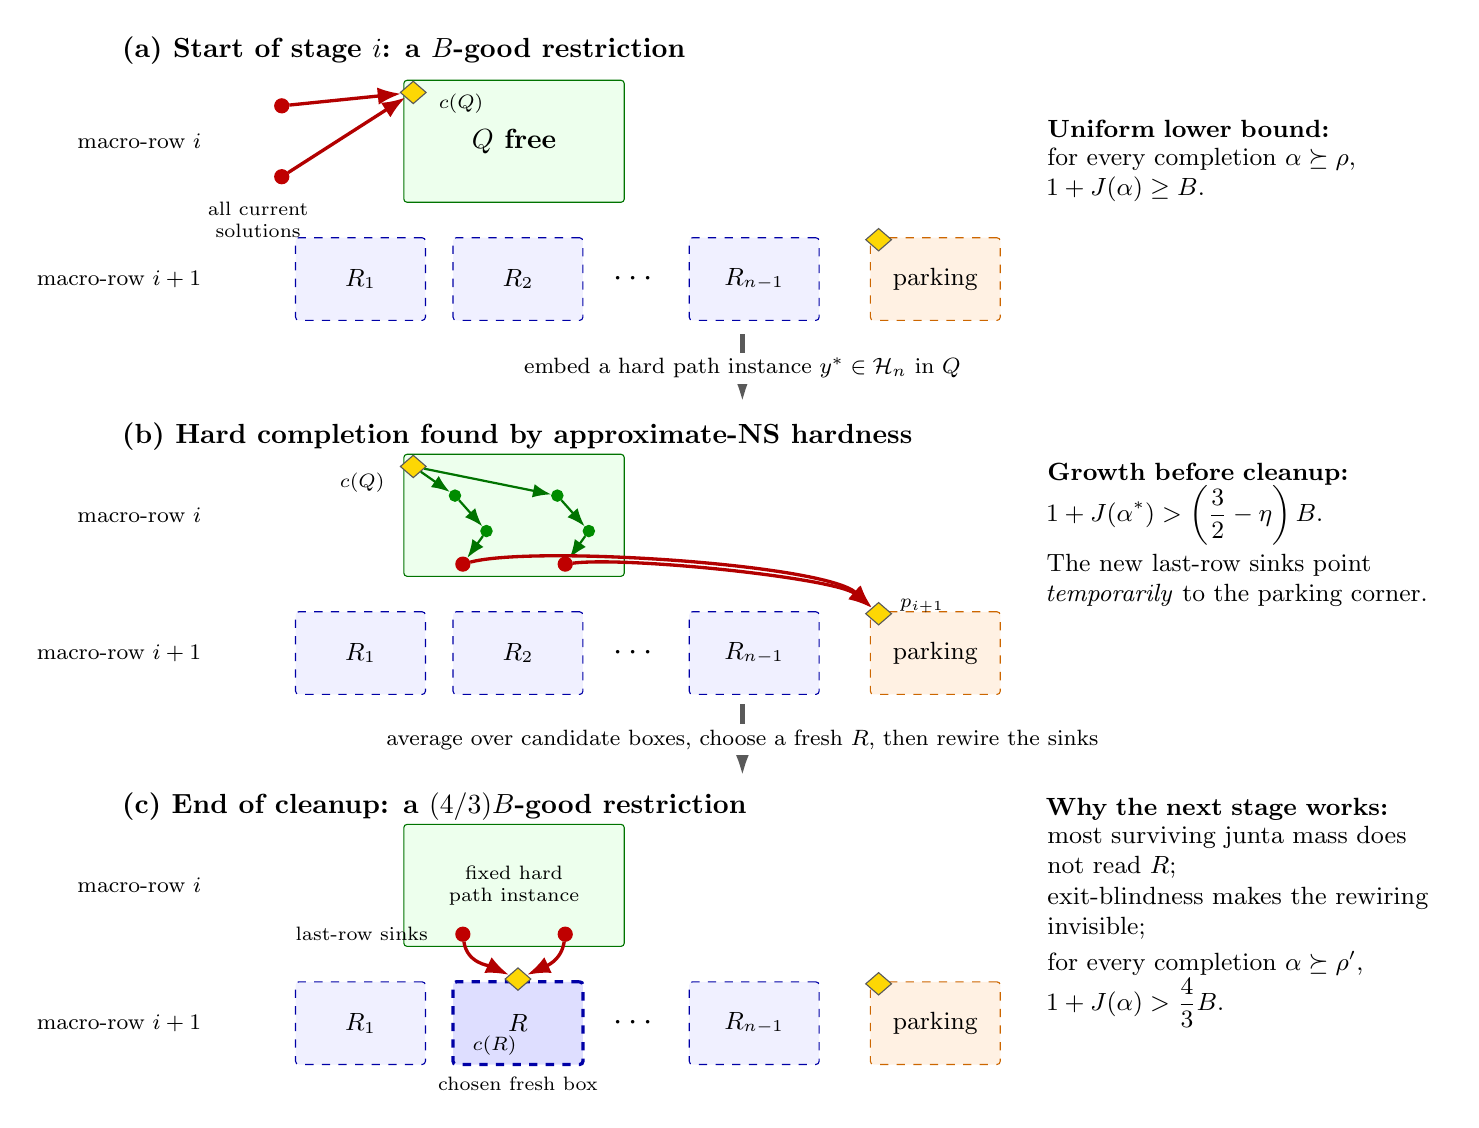
\begin{tikzpicture}[
  font=\small,
  >=Latex,
  candidate/.style={draw=blue!65!black, dashed, rounded corners=1.2pt,
    fill=blue!6, minimum width=1.65cm, minimum height=1.05cm},
  selected/.style={candidate, very thick, fill=blue!13},
  current/.style={draw=green!45!black, rounded corners=1.2pt,
    fill=green!7, minimum width=2.8cm, minimum height=1.55cm},
  parking/.style={draw=orange!80!black, dashed, rounded corners=1.2pt,
    fill=orange!11, minimum width=1.65cm, minimum height=1.05cm},
  sink/.style={circle, fill=red!75!black, draw=red!75!black, inner sep=1.8pt},
  inode/.style={circle, fill=green!55!black, draw=green!55!black, inner sep=1.45pt},
  corner/.style={diamond, aspect=1.15, fill=yellow!75!orange, draw=black!65,
    inner sep=2.2pt},
  flow/.style={->, thick, draw=green!45!black},
  sol/.style={->, very thick, draw=red!70!black},
  transition/.style={->, ultra thick, draw=black!65}
]

% ================================================================
% (a) B-good restriction
% ================================================================
\begin{scope}[yshift=9.3cm]
  \node[font=\bfseries,anchor=west] at (0,2.25) {(a) Start of stage $i$: a $B$-good restriction};

  \node[font=\footnotesize,anchor=east] at (1.25,1.1) {macro-row $i$};
  \node[current] (Qa) at (5.1,1.1) {};
  \node[font=\bfseries] at (5.1,1.1) {$Q$ free};
  \node[corner] (ca) at (3.82,1.72) {};
  \node[font=\scriptsize,anchor=west] at (4.02,1.58) {$c(Q)$};

  \node[sink] (ua1) at (2.15,1.55) {};
  \node[sink] (ua2) at (2.15,0.65) {};
  \draw[sol] (ua1) -- (ca);
  \draw[sol] (ua2) -- (ca);
  \node[font=\scriptsize,align=center] at (1.85,0.10) {all current\\solutions};

  \node[font=\footnotesize,anchor=east] at (1.25,-0.65) {macro-row $i+1$};
  \node[candidate] at (3.15,-0.65) {$R_1$};
  \node[candidate] at (5.15,-0.65) {$R_2$};
  \node[font=\large] at (6.65,-0.65) {$\cdots$};
  \node[candidate] at (8.15,-0.65) {$R_{n-1}$};
  \node[parking] (Pa) at (10.45,-0.65) {parking};
  \node[corner] at (9.73,-0.15) {};

  \node[align=left,anchor=west,text width=5.0cm] at (11.75,0.85)
    {\textbf{Uniform lower bound:}\\[-1pt]
     for every completion $\alpha\succeq\rho$,\\
     $\displaystyle 1+J(\alpha)\ge B$.};
\end{scope}

% transition 1
\draw[transition] (8.0,7.95) -- (8.0,7.10);
\node[fill=white,inner sep=2pt,align=center,font=\footnotesize] at (8.0,7.52)
  {embed a hard path instance $y^*\in\mathcal H_n$ in $Q$};

% ================================================================
% (b) hard completion, parking corner
% ================================================================
\begin{scope}[yshift=4.55cm]
  \node[font=\bfseries,anchor=west] at (0,2.1) {(b) Hard completion found by approximate-NS hardness};

  \node[font=\footnotesize,anchor=east] at (1.25,1.1) {macro-row $i$};
  \node[current] (Qb) at (5.1,1.1) {};
  \node[corner] (cb) at (3.82,1.72) {};
  \node[font=\scriptsize,anchor=east] at (3.58,1.52) {$c(Q)$};

  % two schematic paths inside the current box
  \node[inode] (b11) at (4.35,1.35) {};
  \node[inode] (b12) at (4.75,0.90) {};
  \node[sink]  (sb1) at (4.45,0.48) {};
  \node[inode] (b21) at (5.65,1.35) {};
  \node[inode] (b22) at (6.05,0.90) {};
  \node[sink]  (sb2) at (5.75,0.48) {};
  \draw[flow] (cb) -- (b11);
  \draw[flow] (b11) -- (b12);
  \draw[flow] (b12) -- (sb1);
  \draw[flow] (cb) -- (b21);
  \draw[flow] (b21) -- (b22);
  \draw[flow] (b22) -- (sb2);

  \node[font=\footnotesize,anchor=east] at (1.25,-0.65) {macro-row $i+1$};
  \node[candidate] at (3.15,-0.65) {$R_1$};
  \node[candidate] at (5.15,-0.65) {$R_2$};
  \node[font=\large] at (6.65,-0.65) {$\cdots$};
  \node[candidate] at (8.15,-0.65) {$R_{n-1}$};
  \node[parking] (Pb) at (10.45,-0.65) {parking};
  \node[corner] (pb) at (9.73,-0.15) {};
  \node[font=\scriptsize,anchor=west] at (9.88,-0.05) {$p_{i+1}$};
  \draw[sol] (sb1) .. controls (5.35,0.72) and (9.05,0.48) .. (pb);
  \draw[sol] (sb2) .. controls (6.55,0.58) and (9.20,0.30) .. (pb);

  \node[align=left,anchor=west,text width=5.0cm] at (11.75,0.85)
    {\textbf{Growth before cleanup:}\\[-1pt]
     $\displaystyle 1+J(\alpha^*)>\left(\frac32-\eta\right)B$.\\[2pt]
     The new last-row sinks point\\
     \emph{temporarily} to the parking corner.};
\end{scope}

% transition 2
\draw[transition] (8.0,3.25) -- (8.0,2.35);
\node[fill=white,inner sep=2pt,align=center,font=\footnotesize] at (8.0,2.80)
  {average over candidate boxes, choose a fresh $R$, then rewire the sinks};

% ================================================================
% (c) next good restriction
% ================================================================
\begin{scope}[yshift=0cm]
  \node[font=\bfseries,anchor=west] at (0,1.95) {(c) End of cleanup: a $(4/3)B$-good restriction};

  \node[font=\footnotesize,anchor=east] at (1.25,0.95) {macro-row $i$};
  \node[current] (Qc) at (5.1,0.95) {};
  \node[font=\scriptsize,align=center] at (5.1,0.95) {fixed hard\\path instance};
  \node[font=\scriptsize,anchor=east] at (4.13,0.33) {last-row sinks};
  \node[sink] (sc1) at (4.45,0.33) {};
  \node[sink] (sc2) at (5.75,0.33) {};

  \node[font=\footnotesize,anchor=east] at (1.25,-0.80) {macro-row $i+1$};
  \node[candidate] at (3.15,-0.80) {$R_1$};
  \node[selected] (Rc) at (5.15,-0.80) {$R$};
  \node[font=\scriptsize,anchor=north] at (5.15,-1.36) {chosen fresh box};
  \node[corner] (cR) at (5.15,-0.24) {};
  \node[font=\scriptsize,anchor=west] at (4.45,-1.08) {$c(R)$};
  \node[font=\large] at (6.65,-0.80) {$\cdots$};
  \node[candidate] at (8.15,-0.80) {$R_{n-1}$};
  \node[parking] at (10.45,-0.80) {parking};
  \node[corner] at (9.73,-0.30) {};

  \draw[sol] (sc1) to[out=-82,in=155] (cR);
  \draw[sol] (sc2) to[out=-98,in=25] (cR);

  \node[align=left,anchor=west,text width=5.0cm] at (11.75,0.60)
    {\textbf{Why the next stage works:}\\[-1pt]
     most surviving junta mass does not read $R$;\\
     exit-blindness makes the rewiring invisible;\\[2pt]
     for every completion $\alpha\succeq\rho'$,\\
     $\displaystyle 1+J(\alpha)>\frac43B$.};
\end{scope}

\end{tikzpicture}%
}
\caption{\textbf{The geometry of one amplification stage.}
At the start, a restriction $\rho$ leaves exactly the variables of an empty candidate
box $Q$ unset, all current solutions point to $c(Q)$ in its null completion, and the
lower bound $1+J\ge B$ holds uniformly over every completion $\alpha\succeq\rho$.
A hard $\SoPL_n$ completion inside $Q$ forces growth to more than
$(3/2-\eta)B$; its last-row sinks are first routed to the reserved parking corner.
Only after this completion is fixed do we average over the candidate boxes in the
next macro-row and choose a box $R$ avoided by almost all relevant junta mass.  We
then redirect the sinks to $c(R)$ and unset exactly the variables of $R$.
Exit-blindness preserves the surviving junta values, while $R$ is free in the new
restriction, so the result is a $(4/3)B$-good restriction.  This is exactly the transition proved in
Lemma~\ref{lem:one-step-amplification}.  The drawing is schematic and does not show
literal grid dimensions.}
\label{fig:good-state-amplification}
\end{figure}

Figure~\ref{fig:good-state-amplification} also explains why the parking corner is useful:
it separates two choices that must be made in this order.  We first use the hardness
argument to choose the hard completion $\alpha_{y^*}$; only afterwards do we choose
the fresh box $R$ by averaging, redirect the sinks to $c(R)$, and form the next
restriction $\rho'$.

\subsection{The hardness input}

\begin{theorem}[Approximate-NS hardness of $\SoPL$; external input]\label{thm:sopl}
There exists a constant $a>0$ such that every $1/2$-approximate Nullstellensatz
refutation over $\mathbb R$ of the standard binary encoding of $\SoPL_n$ has degree
at least $n^a$.

More explicitly, if $\{B_D(y)=0\}$ are the multilinear clause-falsification
polynomials for $\SoPL_n$, there do not exist polynomials $p_D$ of total proof degree
below $n^a$ such that
\[
  \frac12\le \sum_D p_D(y)B_D(y)\le\frac32
\]
for every Boolean assignment $y$.
\end{theorem}

This is Lemma~1 of~\cite{GHJMPRT}.  We use only the following support-local
consequence of its proof.  Let $\mathcal H_n$ be the support of the randomized
reduction used there.  Every $y\in\mathcal H_n$ is a disjoint union of directed paths
crossing all $n$ rows, one path starts at the distinguished node, and the only
$\SoPL$ solutions are active sinks on the last row $\{n\}\times[n]$.

\begin{corollary}[Hardness already on the path family]\label{cor:sopl-path}
There is a constant $a>0$ such that the following holds.  Suppose
\[
  Q(y)=\sum_D p_D(y)B_D(y)
\]
satisfies
\[
  \frac12\le Q(y)\le\frac32
  \qquad\text{for every }y\in\mathcal H_n.
\]
Then the proof degree of $Q$ is at least $n^a$.
\end{corollary}

\begin{proof}
This is exactly the support used in the proof of~\cite[Lemma~1]{GHJMPRT}; we recall
why no other inputs are needed.  Their randomized reduction maps an
$(n-1)$-bit input $z$ to a $\SoPL_n$ instance consisting of $1+|z|$ disjoint paths,
then independently permutes the nodes within each nonfirst row.  Hence every output
belongs to $\mathcal H_n$ and all its solutions are active sinks on the last row.

There is one harmless normalization to make explicit.  Suppose
\[
  Q_0(y)=\sum_D p_D(y)B_D(y),\qquad
  |Q_0(y)-1|\le \frac12\quad(y\in\mathcal H_n),
\]
has proof degree $k$.  Define recursively
\[
  Q_{s+1}:=Q_s(2-Q_s)=1-(Q_s-1)^2.
\]
Then $Q_s$ remains in the ideal generated by the same axiom polynomials, since if
$Q_s=\sum_D p_D^{(s)}B_D$, then
\[
  Q_{s+1}=\sum_D p_D^{(s)}(2-Q_s)B_D.
\]
Its proof degree is at most twice that of $Q_s$, while on $\mathcal H_n$
\[
  |Q_{s+1}-1|=|Q_s-1|^2.
\]
After three iterations the error is at most $2^{-8}<0.01$ and the proof degree is at
most $8k$.  Thus the small-error hypothesis used inside the proof of
\cite[Lemma~1]{GHJMPRT} may be assumed without ever evaluating the certificate outside
$\mathcal H_n$.

Now apply the randomized reduction from that proof to $Q_3$.  Their polynomial
$q(y,u)$ selects the summand belonging to the planted last-row sink $u$.  The
local-indistinguishability argument compares the actual planted-sink distribution with
the distribution that, conditioned on $y$, chooses $u$ uniformly from the last-row
sinks.  Every instance $y$ at which the certificate is evaluated belongs to
$\mathcal H_n$.  Consequently the same argument yields an
$O(k\log n)$-degree polynomial approximating $\operatorname{OR}_{n-1}$ (the constant
factor $8$ is immaterial).  The $\Omega(\sqrt n)$ approximate-degree lower bound for
OR gives $k\ge n^a$ for some absolute $a>0$, after decreasing $a$ to absorb the
$O(\log n)$ factor.
\end{proof}

By decreasing the constant if necessary, we henceforth take the exponent in
Corollary~\ref{cor:sopl-path} to satisfy $0<a<1$.

The binary CNF for $\SoD_{n^2}$ has $O(n^4\log n)$ variables, polynomially many
clauses, and width $O(\log n)$.  We use its canonical search-CNF encoding: every
clause $C$ carries a fixed output label $o(C)$, and falsifying $C$ certifies that
$o(C)$ is a valid $\SoD$ solution.

\subsection{Cleaning the conical junta}

It is convenient to regard a term of a conical junta as a partial Boolean assignment.
A term \emph{reads a node} if it reads at least one bit of that node's binary datum.
Relative to the box decomposition above, call a term \emph{clean} if it has the
following three properties.
\begin{enumerate}[label=(\roman*)]
\item \emph{Node-complete:} whenever it reads one bit of a node datum, it reads the
entire $O(\log n)$-bit datum.
\item \emph{Exit-curious:} if it reads a node on the bottom row of a box $Q_{i,j}$,
$i<n$, and fixes that active node's nonnull successor to one of the designated exit
corners
\[
  p_{i+1},c_{i+1,1},\ldots,c_{i+1,n-1},
\]
then it also reads the full datum at that successor node.
\item \emph{Nonwitnessing:} its partial assignment does not already certify a
violated $\SoD$ axiom.
\end{enumerate}

\begin{lemma}[Cleaning lemma]\label{lem:cleaning}
Suppose, pointwise on the Boolean cube,
\[
  P=1+J+E,
\]
where $P$ is in the $\SoD$ axiom ideal with proof degree at most $d$, and $J$ is a
conical junta of degree at most $d$.  Then there are $\widetilde P,\widetilde J$ such
that
\[
  \widetilde P=1+\widetilde J+E,
\]
$\widetilde P$ is still in the $\SoD$ axiom ideal, every term of $\widetilde J$ is
clean, and
\[
  0\le \widetilde J(x)\le J(x)
  \qquad\text{for every Boolean }x.
\]
Moreover both the proof degree of $\widetilde P$ and the degree of
$\widetilde J$ are at most
\[
  d'=O(d\log n).
\]
\end{lemma}

\begin{proof}
First make every term node-complete by repeatedly using
$t=tx_j+t(1-x_j)$ for the unread bits of every node datum touched by $t$.  This
preserves the represented function and nonnegativity and costs an $O(\log n)$ factor
in degree.

Next enforce exit-curiosity.  Once a term is node-complete, every bottom-row node it
reads has a fully specified successor.  Whenever that successor is one of the
specified exit corners, split the term on the $O(\log n)$ bits of the datum at that
corner.  There is at most one such added node record for each already read bottom-row
record, so this changes the degree only by a constant factor after node completion.

Finally remove witnessing terms.  If a term $t$ of coefficient $\alpha\ge0$ certifies
a violated axiom with falsification monomial $A_C$, then in the Boolean quotient
$t=q_CA_C$ for a term $q_C$, with
$\deg(q_CA_C)\le\deg t$.  Replace
\[
  J\leftarrow J-\alpha t,
  \qquad
  P\leftarrow P-\alpha q_CA_C.
\]
The identity $P=1+J+E$ is preserved pointwise, $P$ remains in the axiom ideal, and no
degree increases.  Repeating this for all witnessing terms gives the claim.
\end{proof}

The sole purpose of exit-curiosity is the following simple invariance statement.

\begin{lemma}[Exit-blindness]\label{lem:exit-blindness}
Let $t$ be a clean term.  Let $U$ be a set of active nodes on the bottom row of one
box, and let $r,s$ be two designated exit corners in the next macro-row whose node
data are both null.  Suppose two $\SoD$ assignments $x^{(r)}$ and $x^{(s)}$ differ
only in that every node of $U$ points to $r$ in $x^{(r)}$ and to $s$ in $x^{(s)}$.
Then
\[
  t(x^{(r)})=t(x^{(s)}).
\]
\end{lemma}

\begin{proof}
If the two values differed, then on the assignment where $t=1$ the term would have to
read some rewired node $u\in U$.  Node-completeness makes $t$ see that $u$ is active
and has the corresponding nonnull successor.  Exit-curiosity then makes $t$ read the
full datum at that successor, which is null.  Thus $t$ certifies an active node whose
successor is inactive, hence certifies a violated $\SoD$ axiom.  This contradicts the
nonwitnessing property.
\end{proof}

\subsection{The only transfer statement needed in a stage}

Let $Q$ be a candidate $n\times n$ box with top-left corner $c$.  Given a $\SoPL_n$
input $y$, the \emph{active-edge embedding} into $Q$ makes an internal node $u$ point
to $v$ precisely when the successor and predecessor pointers of $y$ certify the active
edge $u\to v$; otherwise its successor is null.  Last-row active sinks are made to
point to a specified inactive exit corner outside $Q$.

\begin{lemma}[Stage restriction to $\SoPL$]\label{lem:stage-restriction}
Fix all data outside a candidate box $Q$, set all nodes of $Q$ to null, and let $c$ be
its top-left corner.  Assume that the only $\SoD$ solutions outside $Q$ form a
possibly empty set $U$ of active nodes, each pointing to $c$.  If $Q$ contains the
distinguished $\SoD$ node, assume that node is $c$.  Let $p$ be an inactive designated
exit corner outside $Q$.

For a $\SoPL_n$ input $y$, let $\alpha_y$ be the total assignment obtained by the
active-edge embedding into $Q$, with every active last-row sink pointing to $p$.  If
\[
  P(x)=\sum_C r_C(x)A_C(x)
\]
has proof degree at most $d'$, then
\[
  P(\alpha_y)=\sum_D \widehat r_D(y)B_D(y)
  \tag{6.1}\label{eq:stage-restriction}
\]
is an actual Nullstellensatz combination of the canonical $\SoPL_n$ axiom
polynomials, of proof degree $O(d'\log n)$.
\end{lemma}

\begin{proof}
We first check the local search reduction.  Every target bit is determined by a
constant number of binary successor/predecessor pointers, hence by $O(\log n)$ bit
queries.  If $c$ is inactive, every old solution in $U$ remains a $\SoD$ solution and
maps to the inactive distinguished-source solution of $\SoPL$.  If $c$ is active,
those old solutions disappear.  A solution created inside $Q$ is either an internal
active node whose successor became inactive, which maps to the corresponding proper
sink of $\SoPL$, or a last-row active node pointing to the inactive exit corner $p$,
which maps to that last-row sink of $\SoPL$.  Changing the variables in $Q$ cannot create any further
solution in the fixed outside part: the only outside nodes whose solution status can
change are nodes pointing into $Q$, and by hypothesis all such old solutions point to
$c$.  Thus a falsified target clause can be mapped to a falsified source clause using
$O(\log n)$ additional queries.

For completeness, we record why this semantic formulation gives the syntactic
identity \eqref{eq:stage-restriction}.  Fix a target clause $C$ of width $w_C$.
A decision tree of depth $O(w_C\log n)$ determines whether $C$ is falsified and, on
every falsifying leaf, outputs a source clause $D$ falsified throughout that leaf.
The conjunction $m_\ell$ of the queried literals on such a leaf factors as
$m_\ell=q_\ell B_D$.  Summing the disjoint falsifying leaves gives
\[
  A_C(\alpha_y)=\sum_D q_{C,D}(y)B_D(y),
  \qquad
  \deg(q_{C,D}B_D)=O(w_C\log n).
\]
Now normalize each multiplier $r_C$ by restricting the variables of $C$ to their
unique falsifying assignment.  In the Boolean quotient this does not change
$r_CA_C$; if the normalized multiplier has degree $k_C$, then
$k_C+w_C\le d'$.  Under the embedding $y\mapsto\alpha_y$, a degree-$k_C$ monomial acquires degree at most
$O(k_C\log n)$.  Hence every resulting summand has degree
$O((k_C+w_C)\log n)=O(d'\log n)$, proving \eqref{eq:stage-restriction}.
\end{proof}

\subsection{Good restrictions and one-step amplification}

After cleaning, fix the resulting conical junta $J$.  Let $V$ be the set of Boolean
variables of the $\SoD_{n^2}$ encoding, and let $V(Q)\subseteq V$ be the variables
belonging to the node records of a box $Q$.  We use the standard restriction notation
\[
  \rho\in\{0,1,*\}^{V},
  \qquad
  \operatorname{dom}(\rho):=\{v\in V:\rho(v)\neq *\}.
\]
A total assignment $\alpha\in\{0,1\}^{V}$ is a \emph{completion} of $\rho$, written
$\alpha\succeq\rho$, if $\alpha(v)=\rho(v)$ for every
$v\in\operatorname{dom}(\rho)$.  If the unset variables of $\rho$ are exactly
$V(Q)$, let $\rho^{0}$ denote the \emph{null completion} obtained by assigning the
null node record to every node of $Q$.

If $Q=Q_{i,j}$ is a candidate box in macro-row $i$, let $c(Q)=c_{i,j}$.

\begin{definition}[$B$-good restriction]\label{def:good-state}
Let $B\ge1$.  A pair $(\rho,Q)$, where $Q$ is a candidate box in macro-row $i$ and
\[
  V\setminus\operatorname{dom}(\rho)=V(Q),
\]
is \emph{$B$-good} if:
\begin{enumerate}[label=(G\arabic*)]
\item In the null completion $\rho^{0}$, the box $Q$ and every node in all later
macro-rows $i+1,\ldots,n$ are null.  Moreover, the only $\SoD$ solutions outside $Q$
form a possibly empty set of active nodes, all pointing to the inactive corner
$c(Q)$.  In the initial restriction with $Q=Q_{1,1}$, this set is empty and $c(Q)$ is
the distinguished $\SoD$ node.
\item For every total completion $\alpha\succeq\rho$,
\[
  1+J(\alpha)\ge B.
  \tag{6.2}\label{eq:good-numerical}
\]
\end{enumerate}
\end{definition}

Thus a good restriction packages both pieces of information needed for the next
stage: its null completion has the correct outside configuration for the $\SoPL$
embedding, while the lower bound on $1+J$ holds uniformly over every completion of
the restriction.

\begin{lemma}[One-step amplification]\label{lem:one-step-amplification}
Assume, pointwise on the Boolean cube,
\[
  P=1+J+E,
\]
where every term of $J$ is clean, $P$ has proof degree at most $d'$, and
$0\le E\le\eta$ with $\eta\le10^{-2}$.  Assume also
\[
  O(d'\log n)<n^a,
  \qquad
  d'\le\frac n{100},
  \tag{6.3}\label{eq:one-step-degree}
\]
where $a$ is from Corollary~\ref{cor:sopl-path}.

If $(\rho,Q)$ is a $B$-good restriction in macro-row $i<n$, then there exist a
candidate box $R$ in macro-row $i+1$ and a restriction $\rho'$ such that
$(\rho',R)$ is $\frac43B$-good.
\end{lemma}

\begin{proof}
Let $p=p_{i+1}$ be the parking corner in the next macro-row.  For a $\SoPL_n$
input $y$, let $\alpha_y\succeq\rho$ be the total completion obtained by assigning
the variables of $Q$ according to the active-edge embedding of $y$ and making every
active last-row sink point temporarily to $p$.  The structural part of goodness,
applied to the null completion $\rho^0$, allows us to apply
Lemma~\ref{lem:stage-restriction}, so
\[
  P(\alpha_y)=\sum_D\widehat r_D(y)B_D(y)
  \tag{6.4}\label{eq:restricted-representation}
\]
has proof degree $O(d'\log n)<n^a$.

For every $y\in\mathcal H_n$, we have $\alpha_y\succeq\rho$, and therefore the
numerical part of goodness together with $E\ge0$ gives
\[
  \frac{P(\alpha_y)}{B}
  =\frac{1+J(\alpha_y)+E(\alpha_y)}{B}\ge1.
\]
If this quantity were at most $3/2$ for every $y\in\mathcal H_n$, then
\eqref{eq:restricted-representation}, divided by $B$, would contradict
Corollary~\ref{cor:sopl-path}.  Hence some $y^*\in\mathcal H_n$ satisfies
\[
  P(\alpha_{y^*})>\frac32B.
\]
Put $\alpha^*:=\alpha_{y^*}$.  Since $E(\alpha^*)\le\eta$ and $B\ge1$,
\[
  1+J(\alpha^*)>
  \left(\frac32-\eta\right)B.
  \tag{6.5}\label{eq:growth-before-fresh-box}
\]
Because $y^*\in\mathcal H_n$ is a disjoint union of complete paths, it has no
internal proper-sink solutions; its only solutions are its active last-row sinks.

Now choose the next box.  Let $R$ range uniformly over the $n-1$ candidate boxes in
macro-row $i+1$.  For each such $R$, let $J^{\neg R}$ be the sum of those terms of
$J$ that read no node of $R$.  A degree-$d'$ term can meet at most $d'$ candidate
boxes, so
\[
  \Pr_R[t\text{ avoids }R]\ge1-\frac{d'}{n-1}\ge0.98.
\]
Therefore
\[
\begin{aligned}
  \mathbb E_R\bigl[1+J^{\neg R}(\alpha^*)\bigr]
  &\ge
  \left(1-\frac{d'}{n-1}\right)(1+J(\alpha^*))\\
  &>0.98\left(\frac32-\eta\right)B
  >\frac43B.
\end{aligned}
\]
Choose a candidate box $R$ attaining at least this average, and let $c(R)$ be its
corner.

Redirect every active last-row sink of the embedded copy from the parking corner $p$
to $c(R)$, leaving $R$ itself null, and call the resulting total assignment $\beta$.
By Lemma~\ref{lem:exit-blindness}, every clean term has the same value before and after
this redirection.  In particular
\[
  1+J^{\neg R}(\beta)=1+J^{\neg R}(\alpha^*)>\frac43B.
\]
Define the next restriction $\rho'$ by keeping the values of $\beta$ outside $R$ and
unsetting exactly the variables in $V(R)$:
\[
  \rho'(v):=
  \begin{cases}
    *, & v\in V(R),\\
    \beta(v), & v\notin V(R).
  \end{cases}
\]
For every total completion $\alpha\succeq\rho'$, the assignments $\alpha$ and $\beta$
agree outside $R$.  Since $J^{\neg R}$ reads no variable of $R$,
\[
  1+J(\alpha)
  \ge1+J^{\neg R}(\alpha)
  =1+J^{\neg R}(\beta)
  >\frac43B.
\]
This is the numerical part of $\frac43B$-goodness.

For the structural part, the null completion $(\rho')^0$ is exactly $\beta$.  The
distinguished source of $y^*$ is active, so activating the old corner $c(Q)$ removes
all solutions from the preceding stage.  The path instance $y^*$ has no internal
proper sinks.  After the redirection, its last-row sinks are therefore the only
$\SoD$ solutions, and all of them point to the still-null corner $c(R)$.  The box $R$
and all later macro-rows remain null.  Hence $(\rho',R)$ is $\frac43B$-good.
\end{proof}

\subsection{Iteration}

We can now state and prove the robust amplification lemma in a few lines.

\begin{lemma}[Robust $\SoD$ amplification]\label{lem:robust-sod}
There exist constants $\eta,\gamma>0$ with the following property.

Let $F_n=\SoD_{n^2}$, with axiom polynomials $A_C(x)$ equal to the falsification
monomials of its CNF clauses.  Suppose that on the Boolean cube we have a pointwise
identity
\[
  P(x)=1+J(x)+E(x),
  \tag{6.6}\label{eq:robust-id}
\]
where
\begin{enumerate}[label=(\alph*)]
\item $P$ has a representation
\[
  P=\sum_C r_CA_C
\]
of proof degree at most $d$;
\item $J$ is a conical junta of degree at most $d$;
\item $E$ is an arbitrary function satisfying $0\le E(x)\le\eta$ on the Boolean cube;
\item after the cleaning of Lemma~\ref{lem:cleaning}, the resulting degree $d'$ obeys
\[
  O(d'\log n)<n^a
  \qquad\text{and}\qquad
  d'\le \frac n{100},
  \tag{6.7}\label{eq:degree-embed-condition}
\]
where $a$ is from Corollary~\ref{cor:sopl-path}.  Since $d'=O(d\log n)$, it is enough
that $O(d\log^2n)<n^a$; because $a<1$, this also implies $d'\le n/100$ for all
sufficiently large $n$.
\end{enumerate}
Then
\[
  \max_xJ(x)\ge2^{\gamma n}.
  \tag{6.8}\label{eq:Jlarge}
\]
\end{lemma}

\begin{proof}
Apply Lemma~\ref{lem:cleaning}.  It produces a smaller conical junta
$\widetilde J\le J$ pointwise and a corresponding ideal polynomial
$\widetilde P=1+\widetilde J+E$ of degree at most $d'$.  Rename these
$\widetilde J,\widetilde P$ as $J,P$ for the rest of the proof.

Let $Q_1=Q_{1,1}$, and let $\rho_1\in\{0,1,*\}^{V}$ be the restriction that
leaves exactly the variables in $V(Q_1)$ unset and fixes every variable outside
$Q_1$ to its null value.  Then $(\rho_1,Q_1)$ is $1$-good: its null completion is the
all-null $\SoD$ assignment, there are no solutions outside $Q_1$, every later
macro-row is null, and $1+J(\alpha)\ge1$ for every completion
$\alpha\succeq\rho_1$ because $J\ge0$.

Apply Lemma~\ref{lem:one-step-amplification} successively for macro-rows
$1,2,\ldots,n-1$.  We obtain a good restriction in macro-row $n$ with parameter
\[
  B_n=\left(\frac43\right)^{n-1}.
\]
Its numerical condition already gives, for the null completion of its current restriction,
\[
  1+J(x)\ge\left(\frac43\right)^{n-1}
\]
for some Boolean assignment $x$.  Therefore
\[
  \max_xJ(x)
  \ge\left(\frac43\right)^{n-1}-1
  \ge2^{\gamma n}
\]
for some fixed $\gamma>0$ and all sufficiently large $n$.  Since the original junta
before cleaning dominates the cleaned one pointwise, the same lower bound holds for
the original $J$.
\end{proof}

\begin{remark}
The proof has only one inductive object: a $B$-good restriction.  One stage turns a
$B$-good restriction into a $\frac43B$-good restriction.  The error term is used only through
$0\le E\le\eta$; no degree bound on $E$ is needed.  The hard path family and the
structural part of goodness have two separate roles: they justify the syntactic
restriction to the canonical $\SoPL$ axiom ideal, and they guarantee that after a
stage the only surviving solutions are precisely the sinks redirected to the next
fresh box.
\end{remark}


\section{Proof of the main theorem}\label{sec:main-proof}

Let $S$ be the size of $\Pi$.
By Remark~\ref{rem:inert}, for an absolute encoding constant $c_0$,
\[
  T\le c_0S.
  \tag{7.1}\label{eq:TleS}
\]
For convenience put
\[
  B:=\max\{1,c_0S\}.
\]

Choose $0<\beta<a/2$.  Since $a<1$, for all sufficiently large $n$ this ensures both
\[
  O(n^\beta\log^2 n)<n^a
  \qquad\text{and}\qquad
  O(n^\beta\log n)\le \frac n{100},
  \tag{7.2}\label{eq:degree-choice}
\]
where $a$ is from Corollary~\ref{cor:sopl-path}.

Let $\eta,\gamma$ be the constants from Lemma~\ref{lem:robust-sod}.

There are two cases.

\paragraph{Case 1.}
If
\[
  B\,2^{-\kappa R}>\eta,
\]
then, for all sufficiently large $n$, $2^{-\kappa R}<\eta$, so necessarily
$B=c_0S$.  Hence
\[
  S
  \ge
  c_0^{-1}\eta\,2^{\kappa R}
  =
  2^{\Omega(n^\beta)}.
  \tag{7.3}\label{eq:case1}
\]

\paragraph{Case 2.}
Suppose
\[
  B\,2^{-\kappa R}\le\eta.
\]
Then by \eqref{eq:Ebound},
\[
  0\le E\le\eta.
\]
The degree condition \eqref{eq:degree-choice} lets us apply
Lemma~\ref{lem:robust-sod} to \eqref{eq:master}.  Hence
\[
  \max_zJ(z)\ge2^{\gamma n}.
\]
But by \eqref{eq:Jbound} and \eqref{eq:TleS},
\[
  \max_zJ(z)\le T\le c_0S.
\]
Therefore
\[
  S\ge c_0^{-1}2^{\gamma n}
  \ge2^{\Omega(n^\beta)}.
  \tag{7.4}\label{eq:case2}
\]

Combining the two cases,
\[
  \operatorname{Size}_{\RevRes(\oplus)}(\Psi_n)
  \ge
  2^{\Omega(n^\beta)}.
  \tag{7.5}\label{eq:nlower}
\]

By Lemma~\ref{lem:lift-size}, there is a constant $K$ with
\[
  L_n:=|\Psi_n|\le n^K.
\]
Hence
\[
  n^\beta\ge L_n^{\beta/K},
\]
and so
\[
  \operatorname{Size}_{\RevRes(\oplus)}(\Psi_n)
  \ge
  \exp\bigl(\Omega(L_n^{\beta/K})\bigr).
\]
This proves Theorem~\ref{thm:main}.

\section{Dependency audit and points requiring no hidden assumption}

For clarity, we record exactly where external results enter.

\begin{enumerate}[label=\arabic*.]
\item
The conservation identity \eqref{eq:static} uses only the three reversible
$\RevRes(\oplus)$ rules and is proved directly.

\item
Lemma~\ref{lem:affine-conical} is proved entirely in this note.
The high-rank estimate is also reproved directly for the $3$-bit indexing gadget.
A more general version for balanced stifled gadgets appears in
Bhattacharya--Chattopadhyay--Dvo\v{r}\'ak \cite{BCD}.

\item
The only lower-bound ingredient imported from outside this note is the
randomized reduction/local-indistinguishability argument underlying the
approximate-Nullstellensatz lower bound for $\SoPL_n$ in \cite{GHJMPRT}.
Corollary~\ref{cor:sopl-path} records the support-local form of that lower bound used by the amplification, and Lemma~\ref{lem:stage-restriction} proves the required syntactic degree-preserving transfer under the embedding.

\item
The robust amplification Lemma~\ref{lem:robust-sod} is not quoted as a black box.
Its macro-stage growth and cleanup are the coefficient-growth amplification of
\cite[Section~5.1]{GHJMPRT}.  The present proof retains a uniformly bounded
nonnegative error term, makes the transfer to the canonical $\SoPL$ axiom ideal
explicit, and isolates the path-family support needed by the cleanup.  The original
application converts exponential growth into a Sherali--Adams coefficient lower bound;
here the same growth is combined with $\max J\le O(S)$ to lower-bound the
$\RevRes(\oplus)$ proof size.

\item
No restriction is imposed on the width, rank, depth, or affine complexity of the
$\RevRes(\oplus)$ proof lines.  High-codimension final affine spaces are handled by
Lemma~\ref{lem:high-rank}; low-codimension spaces are handled exactly by the
selector decomposition in Lemma~\ref{lem:affine-conical}.

\item
The lower bound is measured against the actual CNF encoding size.
The constant-size gadget is essential here: a base clause of width $O(\log n)$
expands by only $4^{O(\log n)}=n^{O(1)}$.
\end{enumerate}

\section{A reusable abstract formulation}

The argument can be packaged as the following general criterion.

\begin{theorem}[Abstract criterion]\label{thm:abstract}
Let $F_n$ be polynomial-size CNFs of width $O(\log n)$.
Assume there are constants $a,\eta,\gamma>0$ such that every pointwise identity
\[
  P=1+J+E
\]
with
\begin{itemize}
\item $P$ in the Boolean axiom ideal of $F_n$ with proof degree below $n^a$,
\item $J$ a conical junta of degree below $n^a$,
\item $0\le E\le\eta$,
\end{itemize}
satisfies
\[
  \max J\ge2^{\gamma n}.
\]
Then the constant-size indexing lift $F_n\circ g$ requires
\[
  2^{n^{\Omega(1)}}
\]
size in $\RevRes(\oplus)$, and this is
$\exp(|F_n\circ g|^{\Omega(1)})$ in terms of formula size.
\end{theorem}

\begin{proof}
Repeat the lifting and parameter argument above, using the hypothesis of the theorem in place of the robust coefficient-growth amplification from Section~\ref{sec:base-lb}.
\end{proof}

\nocite{AG}
\bibliographystyle{alpha}
\bibliography{revres_xor_superpoly_lower_bound_alpha}

\end{document}
